\section{Related Work}
\label{sec:related_work}
Our work spans multiple areas of research. We review literature that addresses 
construction of word embeddings and their utility in information retrieval.
\begin{figure}[t]
        \centering
        \includegraphics[width=\linewidth]{elements.pdf}
        \caption{Percentage distribution of the presence of different structural 
elements considered.}
        \label{fig:elements}
\end{figure}
\subsection{Distributional Semantics for IR}
While many word embedding models have been proposed recently, the Continuous 
Bag-of-Words (CBOW) and the Skip-Gram
(SG) architectures proposed by Mikolov et al. \cite{mikolov2013distributed} are 
arguably the most popular. More recently, a theoretical framework was proposed 
which estimates query embedding vectors based on the individual embedding 
vectors of vocabulary terms \cite{zamani2016estimating}. In terms of 
applications, word embeddings have been studied in various IR contexts such as 
term reweighing \cite{zheng2015learning}, cross-lingual retrieval 
\cite{vulic2015monolingual} and short text similarity 
\cite{kenter2015short}. Beyond word co-occurrence, recent studies have also 
explored learning text embeddings from click-through data 
\cite{shen2014learning}, session data \cite{grbovic2015context} and for query 
prefix-suffix pairs \cite{mitra2015query}. Finally, Diaz \textit{et al.} 
\cite{diaz2016query} highlight the value of locally-training word embeddings retrieval. 
We explore the use of embeddings to represent 
contributions from different structural elements comprising document and 
proposing novel ways of leveraging such representations for improved document 
retrieval.

%\subsection{Document Retrieval with embeddings}
\subsection{Document Representations}
Vector based representation of documents is a standard practice in retrieval. 
A document vector simply encapsulates the importance of each 
term in the document and is usually highly dimensional. As a consequence, 
these vectors are sparse. To address the data
sparsity issue, several dimensionality reduction approaches have been proposed 
in the literature. A popular class of
methods is based on linear projection, which projects a high-dimensional vector on to a lower dimensional space. 
A historical approach to linear projection is Principal Component Analysis (PCA) 
\cite{jolliffe1986principal}, which performs a singular value decomposition 
(SVD) on a document matrix D of size n $\times$ m, where each row in D is the 
term vector representation of a document. Latent Semantic Analysis (LSA) 
\cite{deerwester1990indexing} is very similar to PCA but performs the SVD using 
the correlation matrix instead of the covariance matrix, which implies a lower 
computational cost. Other projection models such as Latent Dirichlet Allocation 
(LDA) \cite{blei2003latent} are based on the generative models of text in documents. 
Another approach, named Explicit Semantic Analysis (ESA) 
\cite{gabrilovich2007computing}, represents each document by its similarities to other documents in a collection. 
Using a low domain specificity document collection such 
as Wikipedia, the model has proven to obtain competitive results. Deep 
architectures have been shown to be highly effective in discovering from 
training data the hidden structures and features at different levels of 
abstraction useful for a variety of tasks. Liu \textit{et al.} 
\cite{liu2015representation} propose a representation Learning technique which 
makes use of a Multi-Task Deep Neural Networks for semantic retrieval. Recently, 
Shen \textit{et al.} \cite{shen2014learning} present a series of new latent 
semantic models based on a convolutional neural network (CNN) to learn 
low-dimensional semantic vectors for search queries and Web documents. The 
interested reader is directed to Li \textit{et al.} \cite{li2014semantic} which 
presents a comprehensible survey summarizing different semantic matching 
techniques.
\begin{figure*}[t]
        \centering
        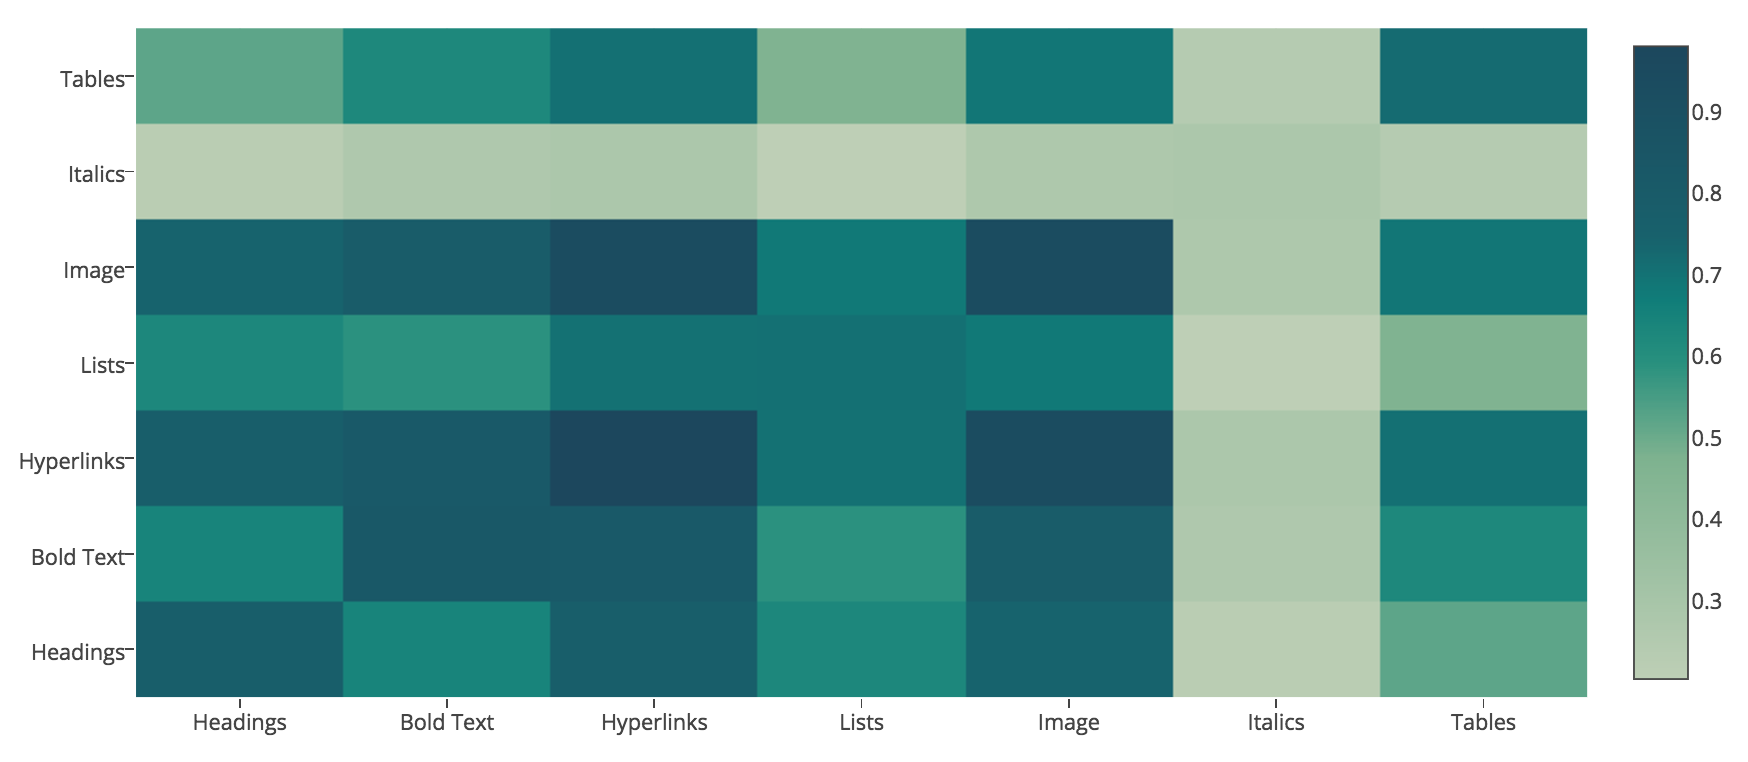
\includegraphics[width=0.8\linewidth]{heatmap.png}
        \caption{Element co-occurrence visualized via heatmap.}
        \label{fig:heatmap}
\end{figure*}
\subsection{Exploiting Document Structure}
Beyond exact and semantic matching of queries and documents for retrieval, the 
use of number of different features and elements have been explored by enhanced 
retrieval techniques. Tombros \textit{et al.} \cite{tombros2005users} 
investigate the criteria used by online searchers  and presented the relative 
utility of features: web page content,
structure and quality and their importance when assessing the relevance of web 
pages for information-seeking tasks. Hui \textit{et al.}\cite{hui2017position} 
consider positional information and propose position-aware representations for 
relevance matching in a neural retrieval framework. Recently  \cite{verma2016obtaining} 
found that presence of structural elements in webpage reduce user's overhead in finding 
required information from a webpage quickly which provides a strong motivation for our work 


